\section{Theory}
\label{sec:theory}
\subsection{Related work}
Motivated by peer-to-peer and ad hoc networks, a considerable number of studies have been done regarding gossip-based algorithms. Convergence and upper bound consensus time have been proven by J.Lavaei and R.Murray in \cite{5929538}. Analytical methods and simulations have been utilized to discuss the relations between performance of gossip protocols and topology of network, namely randomness, connectivity etc. As a subcategory of distributed algorithm different models, such as synchronous and asynchronous models, with or without churn, are discussed in \cite{Lynch:1996:DA:525656}. The optimization of parameters of an asynchronous randomized gossip algorithm for faster convergence is proven to be a semi-definite problem \cite{Boyd2004}.

This study is mainly based on the work of M.Jelasity, A.Montresor and O.Babaoglu \cite{jelasity_gossip-based_2005}, focusing on existing static networks of different topologies \cite{knight_internet_2011}

\begin{figure}[h!]
   \begin{minipage}[t]{0.45\textwidth}
      \vspace{0pt}
      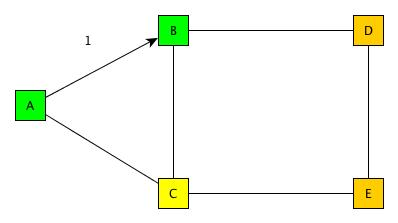
\includegraphics[width=\linewidth]{figures/network_gossip_1.jpg}
      Beginning of message dissemination (a)
   \end{minipage}
   \hfill
   \begin{minipage}[t]{0.45\textwidth}
      \vspace{0pt}
      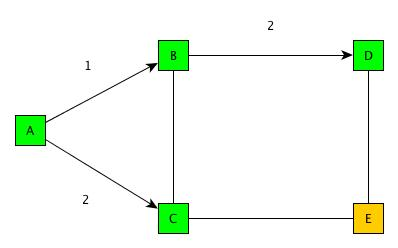
\includegraphics[width=\linewidth]{figures/network_gossip_2.jpg}
      Passing the message (b)
   \end{minipage}
   \vspace{5ex}
     \begin{center}
     \begin{minipage}[c]{0.45\textwidth}
      \vspace{0pt}
      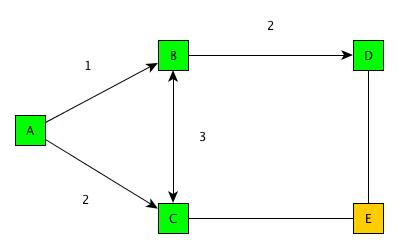
\includegraphics[width=\linewidth]{figures/network_gossip_3.jpg}
      Probable redundant message (c)
   	\end{minipage}
   \end{center}
   \caption{Gossip algorithm evolution epochs}
   \label{fig:epochs}
\end{figure}
\subsection{Gossip-based aggregation}

%TODO: describe the algorithm in details
\subsubsection{Gossip algorithm}
For better understanding of gossip algorithm, we assume a graph as in figure \ref{fig:epochs}. It illustrates a typical message dissemination process applying gossip algorithm. It starts with one node containing the information to be propagated, as in subgraph (a). It randomly chooses one neighbor and send the message. In second epoch, as showed in subgraph (b), this message is passed forward to next hop in the same manner, including the root node. By recursively applying same procedures, the message will be passed through the whole network eventually. Subgraph (c) shows the occurrence of probable redundant packet from node 3 to node 2, who's already aware of the message. Because of randomness of gossip algorithm, complete dissemination can only be achieved at a certain probability within given epochs, which can be denoted as $D(x)=\int_0^x P(\xi)\mathrm{d}\xi$\\

\subsubsection{Aggregation}
% TODO: illustrate aggregation

A simple implementation of synchronous gossip-based aggregation algorithm, inspired by \cite{jelasity_gossip-based_2005} can be illustrated by following pseudo code \ref{code:pseudo}.
\begin{figure}[!h]
\begin{lstlisting}[caption={Pseudo Code for gossip-based aggregation}, label=code:pseudo, mathescape=true, captionpos=b]
$ActiveGossipThread$
$\mbox{for each consecutive } \delta \mbox{ time units at randomly picked time; do}$
    $q \leftarrow GET\_NEIGBOR()$
    $send\_to({state}_{p},$ $q)$
    $state_{q} \leftarrow receive(q)$
    $state_{p} \leftarrow UPDATE(state_{p},$ ${state}_{q})$

$PassiveGossipThread$
$\mbox{while true:}$
    $state_{q} \leftarrow receive(*)$
    $send\_to(state_{p},$ $q)$
    $state_{p} \leftarrow UPDATE(state_{p},$ $state_{q})$
\end{lstlisting}
\end{figure}

Although convergence is proven and expected convergence time can be estimated by probability density function for a certain topology \cite{5929538}, a drawback of probabilistic algorithm comparing to deterministic algorithm is reliability \cite{Lynch:1996:DA:525656}. The value can only be considered as true result at a certain probability. To put this protocol into practice, some extra procedures need to be added. In this study, we leave out the test of correctness inside implementation but try to obtain an empirical criteria according to the result of experiments.

\subsection{Impact of topology toward the performance of aggregation}
A plenty of methods exist to describe overlay topologies of a network, and different representations are used to describe properties of a topology. On the other hand, the performance of gossip-based aggregation is also abstracted differently for specific purpose.

In this study, we firstly focus on investigating the impact of various number of links with the number of nodes unchanged over the performance of gossip-based aggregation algorithm. %Then we try to extract proper parameters representing a unweighted undirected connected graph through applying the definition of entropy presented by \cite{entropy1} and \cite{entropy2} and then we apply inductive research method \cite{portal} to address the relation between entropy and convergence time.
%TODO: describe definition in detail

\subsection{Applying to real network}
In order to apply control variable experiment method, we based our experiment on 4 real network topologies (see figure \ref{fig:graphs}) with same number of nodes (37) and different number of links, as showed in Table \ref{table:network}. %Entropies are also calculated by applying methods presented by \cite{entropy1} (referred in the table as Entropy1) \cite{entropy2} (referred in the table as Entropy2).

\begin{figure}[h!]
   \begin{minipage}[t]{0.45\textwidth}
      \vspace{0pt}
      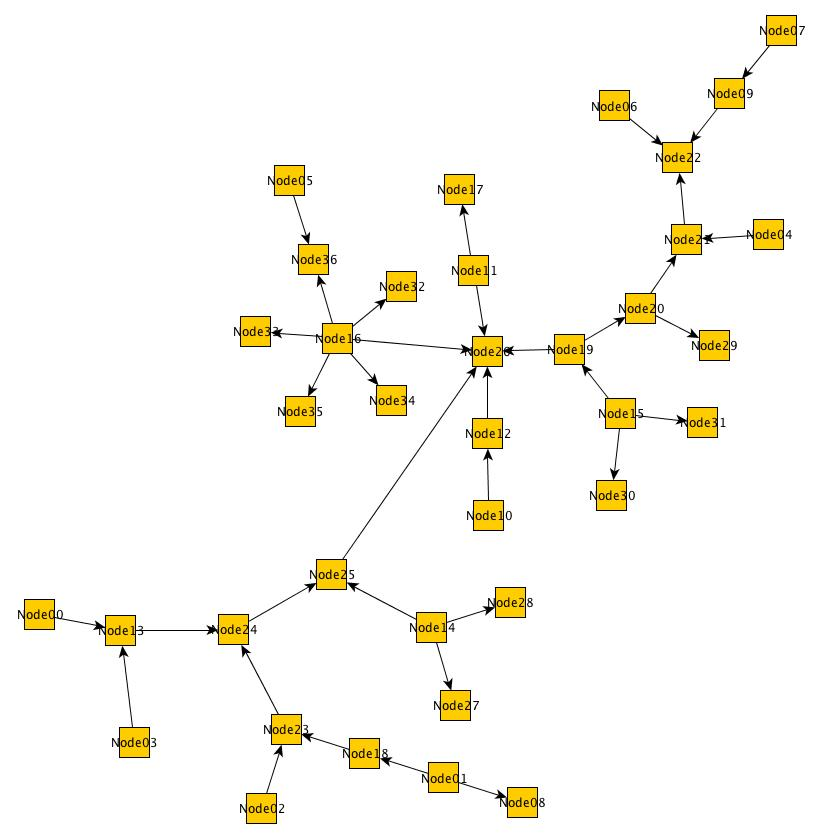
\includegraphics[width=\linewidth]{Reuna.jpg}
      Backbone of Chile (a)
   \end{minipage}
   \hfill
   \begin{minipage}[t]{0.45\textwidth}
      \vspace{0pt}
      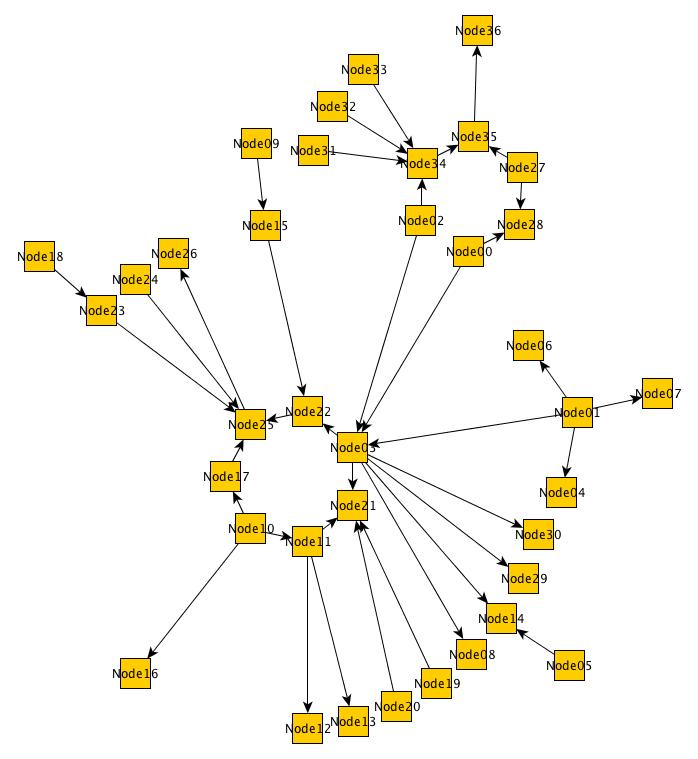
\includegraphics[width=\linewidth]{Bren.jpg}
      Backbone of Bulgaria (b)
   \end{minipage}
   \vspace{4ex}
    \begin{minipage}[c]{0.45\textwidth}
    \vspace{0pt}
    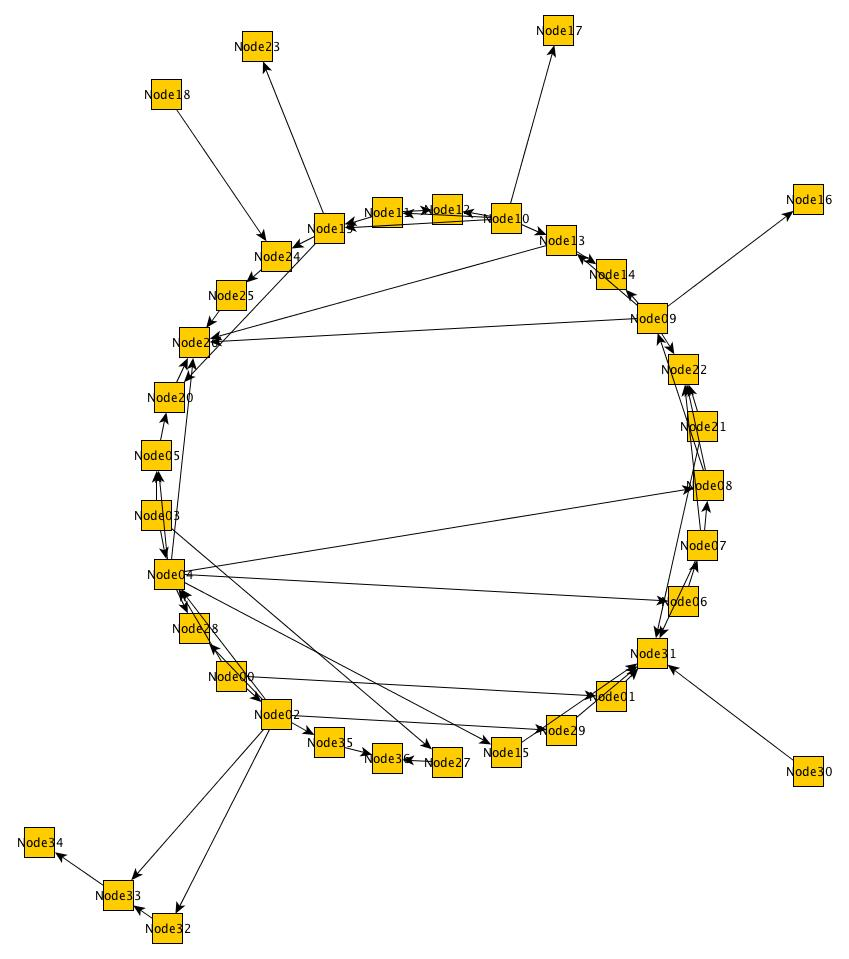
\includegraphics[width=\linewidth]{Geant2010.jpg}
    European transit network (c)
    \end{minipage}
    \begin{minipage}[c]{0.45\textwidth}
    \vspace{0pt}
    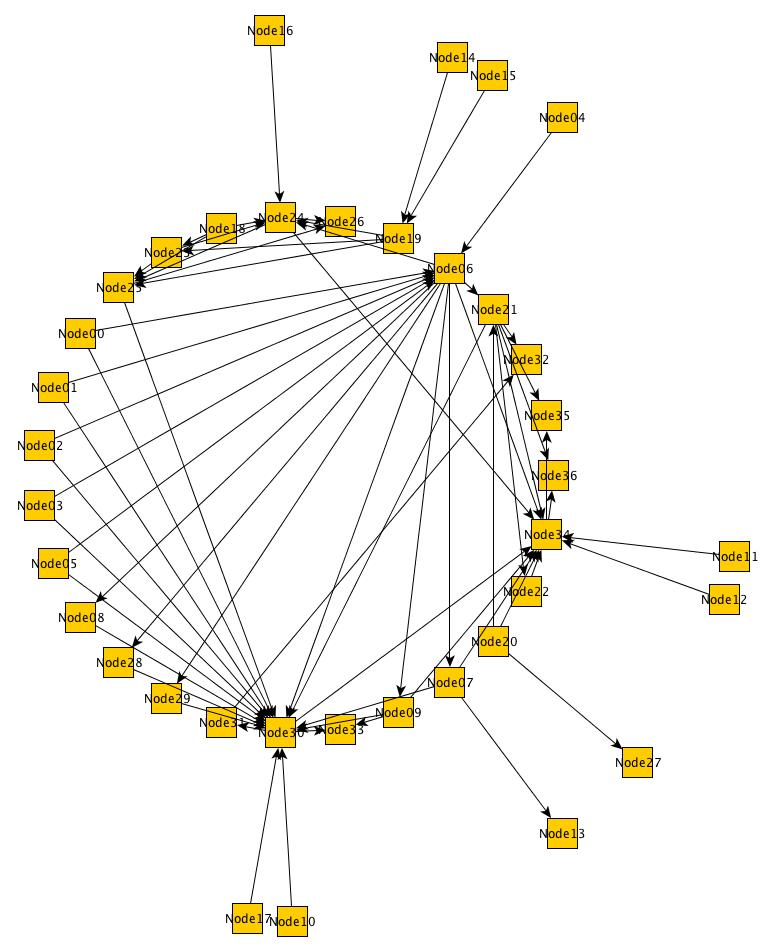
\includegraphics[width=\linewidth]{Iij.jpg}
    Backbone network Japan, USA (d)
    \end{minipage}
   \caption{Different graph topologies (in ring layout)}
   \label{fig:graphs}
\end{figure}
\begin{table}
\centering
\begin{tabular}{lrrcrr}
	\hline
	Name of Network & Year & Country & \# of Links\\% & Entropy1 & Entropy2\\
    \hline
    Reuna & 2010 & Chile & 36\\% & 202.0476 & 0.5164084\\
    BREN & 2010 & Bulgaria & 38\\% & 210.2229 & 0.6214745\\
    Geant & 2010 & Europe & 58\\% & 277.3282 & 1.530375\\
    Iij & 2010 & Japan, USA & 66\\% & 307.2482 & 1.553654\\
    \hline
\end{tabular}
\caption{Topologies under investigation}
\label{table:network}
\end{table}

\subsection{Hypothesis}
%{\it Hypothesis 1.}
In a given network topology $\mathcal{G}=\{\mathcal{E}, \mathcal{V}\}$, the number of links (edges) $N_E$ and convergence time $t$ are positively correlated, with number of nodes (vertices) $N_V$ unchanged.
%{\it Hypothesis 2.} In a given network topology $\mathcal{G}=\{\mathcal{E}, \mathcal{V}\}$, the entropy of this graph $S$ and convergence time $t$ are positively correlated.

\subsection{Research methodology and methods}
We are creating a positivistic investigation grounded in quantitative experiments. With induction in the form of statistical inference, we aim to predict the behavior of the system under question in the boundary of our experimental research.

We clearly distinguish ourselves from realism, as we use network graphs inspired by real networks, but leave it to other research to prove that the experiment is representative of those real networks.

Since we will investigate several existing networks with the same number of nodes (constant) but different number of links (variable), we choose experimental research as our research method.

We will apply inductive reasoning research approach to verify the hypothesis. Since our unique contribution is an investigation of real network rather than a theoretical proof, deductive reasoning research approach does not fit our goal properly.
%We will run our experiment multiple times to collect data and based on the observation of these phenomena we can obtain our conclusion.
